

\cs{@gbt @mw}
\subsection{Overview of ManyNames}
\label{sect:mn_overview}

brief summary of lrec paper, shortcoming, what we added

\subsection{Verification of Annotations}
\label{sect:mn_verification}

\mw{Below can be shortened no doubt; but could also be moved to appendix. Plz. let me know what you consider the most appropriate (I'm an ACL noobie).}

Although the initial data gathering phase involved some very basic quality control (detecting repeated names, empty text fields, typos), we had no rigorous way of ascertaining that our participants were providing adequate names for the intended object.
Given our high number of annotators in phase 1 we decided to simply discard names that were entered by only one annotator.
Moreover, for images where all 36 annotators entered the same name we decided to take this name to be adequate. 
That still leaves 19427 images, with on average 4 names each, to be properly verified, which we did as follows.

We conducted a second round of annotation where we asked people whether each name for a given image was adequate and, if not, what type of inadequacy it was.
Moreover, we asked them to indicate which names were likely intended for the same real-world object.
The task interface is shown in figure~\ref{fig:verification-interface} in the appendix.
% \begin{figure*}[t]
% 	\centering
% 	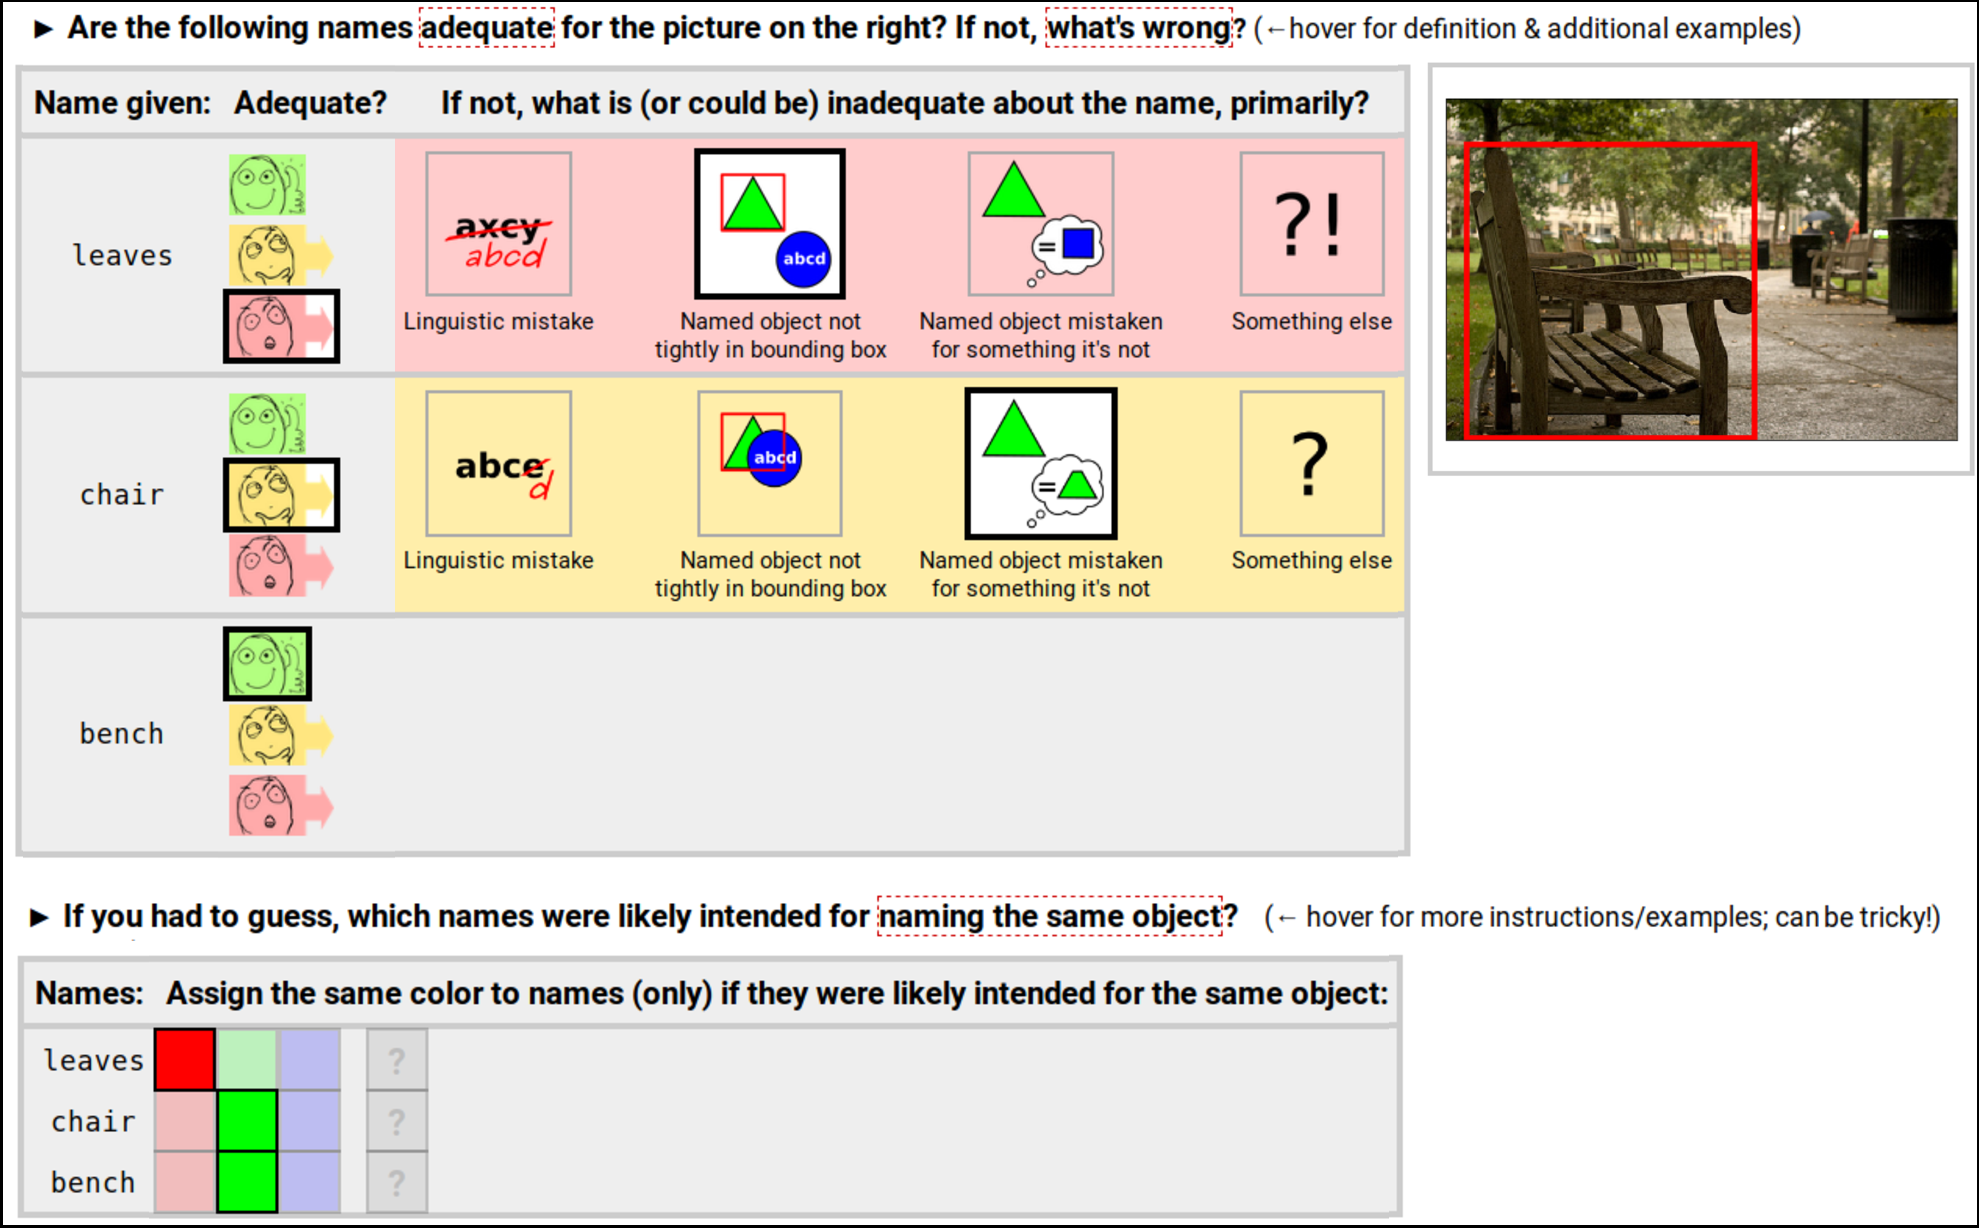
\includegraphics[width=\textwidth]{images/verification-interface.pdf}
% 	\caption{A screenshot of our verification task interface. Up to ten names could be shown for an image in this way (the number of available colors in the second task would increase accordingly).}
% 	\label{fig:verification-interface}
% \end{figure*}
Adequacy was rated on a 3-point scale from ``perfectly adequate'' to ``there may be a (slight) inadequacy'' to ``totally inadequate'', represented by appropriate rage faces.
We provided (and clarified by means of explanation and visual examples) the following definition: \textit{a name is ``adequate'' if there is an object in the image, whose visible parts are tightly circumscribed by the red bounding box, that one could reasonably call by that name}.
When the participant selected slightly or totally inadequate, four additional icons would appear to indicate the type of inadequacy: ``linguistic mistake'', ``named object not tightly in bounding box'', ``named object mistaken for something it's not'', and ``something else''.
We provided detailed instructions and examples at the top, as well as informative hover texts on all the buttons.

Because the quality of the data we gather in this phase will be essential for gaining insight into our data from phase one, as well as for evaluating computational object naming models (section~\ref{sec:experiments}), we set up a rigorous quality control protocol.
Every task included between 10\% and 20\% automatically generated quality control items of various kinds (names for objects in a different image, names for other objects in the same image, WordNet synonyms of given names, inserted typos, and more).
Participants would get a warning if, upon submitting their results, their accuracy on these items was below 90\%, and the advice to not do any more tasks of this type if it was below 80\%.
After every round we blocked annotators with low (<90\%) average accuracy, removed their results from the dataset and republished the relevant tasks to ensure consistent coverage of our data.

We implemented our task on Amazon Mechanical Turk (\url{https://mturk.com}).
We relied on 255 mostly recurring workers, who did a total of 9491 published tasks.
Each task would present the worker with 6 or 7 images, for a total of between 20 and 30 names.
We offered a reward of \$0.50 with an additional bonus of \$0.15 if all control items were answered correctly as extra incentive (which happened about half the time).
Our approach was valued by the workers for the interesting task, natural interface and good reward.

\mw{Maybe the following should go in 3.3 analysis? I think it fits here though.}
We reached high inter-annotator agreement: adequacy judgments (encoded on a scale from 0 to 2) have a standard deviation of 0.19, with the proportion of annotators agreeing on ``adequate'' being 88\%; the proportion of annotators agreeing on inadequacy type (the 4 options) is 86\%, and this agreement is 94\% on the judgments of whether two names were intended for the same object.
Bearing in mind that the latter often required our participants to do some kind of mind-reading -- which object could someone who entered an inadequate name plausibly have in mind? -- this level is agreement is very high.

\mw{Probably the following should go to 3.3 analysis}
For our analysis below we aggregate our judgments of adequacy by taking the mean, and judgments of inadequacy type by taking the majority (also counting ``none'' if there was no inadequacy).
As for the judgments of whether two names were intended for the same object, we use two different types of aggregations, for different purposes.
For evaluating computational object naming models, we want to know primarily whether a name generated by a model could have been intended to name the same object as the entry-level name (i.e., the most frequent name).
This we compute by a simple majority rule: true if name1 and name2 were judged to be for the same object by a majority of annotators, and false otherwise.
However, we are also interested in more general statistics, e.g., the mean number of names per object, and the relative frequencies of names for a given object.
For this, we need to compute clusters of names  (the pairwise majority rule does not result in a proper clustering): as distance between names we use the proportion of annotators saying they do not name the same object, and we perform agglomerative, complete-linkage clustering with a threshold of .5 (i.e., all pairs of names in a cluster must name the same object according to a majority of annotators).
A disadvantage of this (hard) clustering method is that every name can only be in one cluster, i.e., name only one object. \mw{But this is not as bad as it sounds! It's often quite plausible, e.g., that food names the pizza, not the topping!}
This way, our method may slightly underestimate the number of names per object.
(The alternative -- soft clustering, where each name could potentially be in multiple clusters -- risks overestimating the number of named objects in an image.)

\mw{I realize the foregoing is quite cryptical... Sorry no more time to work on this today!}

\subsection{Analysis}
\label{sect:mn_analysis}


\paragraph{Of ManyNames:} 
\cs{+ @sz?}\\
\cs{Here goes what has not been discussed in LREC paper, because it focusses on entry-level names. }
\cs{Results aimed to show that we need \underline{multiple} annotations per object \underline{instance} to get the entry-level name}
\begin{itemize}
	\item Statistics wrt entry-level of object class != entry-level of its instances to (i.e.,\ entry-levels cannot be derived on class-level) \gbt{But, what's an object class in our data? We can't really use collection synsets, can we? Those are not really object classes?} \gbt{UPDATE: We change focus from class to ``entry-level names are instance-specific''. Matthijs is on it.}
	\item Plot of how most frequent name changes in relation to the number of responses collected (e.g., phase 0 vs. 1 vs. 2 vs. 3). (i.e.,\ entry-level names cannot be derived from a few annotators). \gbt{UPDATE:}
          \begin{itemize}
          \item The average change in most frequent name across rounds is 20\% (SD 2.4\%) -- i.e. even having 9 names only assures you to get the entry-level name for 80\% of the objects on average. \gbt{The data would be more compelling if we did proper sampling (samples of 1, 2, 3, ... names). Matthijs is on it. }
          \end{itemize}
	\item Coverage of set of topN MN names (MN442) wrt all VG objects \cs{@\sz} \gbt{According to my data, there are 415 entry-level names (=entry-level names for canonical object; could extend definition to all objects if need be). Are your 442 names the most frequent names for some image? Else, we could do the experiments with the entry-level names as the vocabulary (but it's probably too late now).}
	\item ...
\end{itemize}


\paragraph{Of Verification Annotations}
\cs{@gbt @mw}



\begin{itemize}
	\item ...
	\item ...
	\item For the instances where VG!=topMN: Percentage of instances where the VG name is among the responses of an \textit{alternative object} (as given by clustering).
\end{itemize}


%%% Local Variables:
%%% mode: latex
%%% TeX-master: "acl2020_main"
%%% End:
